\chapter{Application Design, Implementation and Testing}
\label{chap:design_implementation}

\par This chapter covers the design and implementation of the application specified in Chapter~\ref{chap:requirements} and the testing that verifies the core functionality (per-flow classification of submitted traffic). It is organised top-down, starting from the architectural breakdown, moving through each component's design and the implementation choices that turn it into running code, and finishing with the testing strategy and the functional acceptance evidence.

\section{Architectural Overview}
\label{sec:architecture_overview}

\par The system is split into a training subsystem (offline) and a serving subsystem (online), as introduced in Section~\ref{sec:system_specification}. The two are decoupled by a small, well-defined contract: a fixed number of serialised artefacts per trained model variant. This decoupling is deliberate. It lets the training side iterate freely (different splits, granularities, hyperparameters) without forcing changes to the serving code, and it lets the serving code stay tiny and observable.

\subsection{Component Decomposition}
\label{subsec:module_decomposition}

\par The application decomposes into five components, each with a single concern so that a fault is locatable, and the boundary between them is the artefact contract rather than a network protocol or in-process API, which lets the training side be re-run independently of any deployed serving instance and the serving side be reloaded by pointing it at a different artefact directory. The training pipeline handles ingestion, deduplication, per-class subsampling, splitting, scaler and encoder fitting, model training, evaluation, latency benchmarking, and artefact persistence. The inference component loads the scaler, encoder, and weights for a given (split, granularity) variant, preprocesses incoming feature rows, runs the model, and returns labelled predictions with confidences. The capture-to-CSV bridge locates a CICFlowMeter backend, runs it as a subprocess against a packet capture, and returns the path of the feature CSV it produces. The web application discovers the model variants on disk, exposes the user interface, routes uploads through the inference component, and formats the verdicts. Beneath all of these, the project specification fixes the invariants (feature set, split strategies, classification granularities, and modelling constraints) that bind every component.

\subsection{Artefact Contract}
\label{subsec:artefact_contract}

\par The serving subsystem consumes exactly three artefacts per model variant, produced by the training pipeline and read back by the inference component: the fitted feature scaler for the split (one per split, shared across granularities because the input feature space is identical regardless of label encoding), the fitted label encoder for the (split, granularity) pair (one per granularity, because the label set changes), and the trained model weights for that pair.

\par The artefact filenames encode both the split and the granularity in a uniform pattern. As a consequence, the web application can probe the artefact directory at startup, parse each filename, and instantiate one inference component per complete artefact triple it finds, with no hard-coded list of variants. Exposing a newly trained variant in the user interface is therefore purely a question of dropping its three files into the artefact directory and restarting the application.

\section{Data Pipeline Design}
\label{sec:data_pipeline_design}

\par The training data pipeline performs a sequence of deterministic transformations from the raw per-folder CSVs to the train/validation/test tensors that feed the model. Each transformation is a separate pipeline phase so that intermediate state is inspectable.

\subsection{Ingestion and Deduplication}
\label{subsec:ingestion}

\par For each of the attack folders, the pipeline lazily scans every CSV, projects only the feature columns plus a synthetic column that carries the source-capture filename, and concatenates the resulting lazy frames. Materialisation happens only after the projection, so the multi-tens-of-millions-of-rows corpus is never held in memory in its raw width.

\par CICIoT2023 contains a substantial fraction of exact duplicate rows, a known property of the dataset and a recurring concern in the literature. Deduplication is applied immediately after concatenation, before any sampling. Deduplicating before sampling is essential: a folder where most rows are duplicated would otherwise have the same row repeated many times in the sample, which would inflate accuracy on the corresponding test rows. The quantitative impact of each pipeline stage (raw count, duplicates removed, unique rows, sampling cap applied) is reported in Chapter~\ref{chap:results} (Figure~\ref{fig:ingest_waterfall}).

\subsection{Per-Class Subsampling}
\label{subsec:subsampling}

\par After deduplication, every folder whose deduplicated row count exceeds the per-class cap is randomly subsampled to that cap with a fixed seed. This brings the effective training-set size down from tens of millions of rows to a few million while keeping every attack class represented.

\par The cap is set at the high end of the range used in the CICIoT2023 literature. Random sampling is preferred over taking the leading rows of each folder because each attack folder is a chronological concatenation of several capture sessions: the first $N$ rows come almost entirely from the first session, and a leading-rows sample would bias the model toward whatever happened in that opening session.

\subsection{Caching}
\label{subsec:caching}

\par The deduplicated, subsampled, labelled rows are concatenated across folders and written to a single Zstandard-compressed columnar file. Subsequent runs skip ingestion and load from this cache directly. Regeneration is forced by deleting the cache file. This is documented inline so future runs do not silently use a stale cache after sampling logic changes.

\subsection{Cleaning}
\label{subsec:cleaning}

\par The cleaning phase performs three operations on the materialised frame. First, null-label rows are dropped (defensive only; labels come from folder names, so this should be a no-op). Second, infinities are replaced with nulls; the actual median imputation is deferred to after the train/validation/test split so the medians are computed on the training partition only. Third, a $\log(1+x)$ transform is applied to the heavy-tailed continuous features (rates, total bytes, inter-arrival times). Binary protocol and flag indicators are excluded from the log transform.

\subsection{Three Split Strategies}
\label{subsec:split_strategies}

\par Three splitting functions are defined and selected by configuration. Their design follows directly from the requirements in Section~\ref{subsec:pipeline_requirements}.

\par \textbf{Random row split.} Two stratified splits in series produce 70/15/15 train/validation/test partitions, stratified by the fine-grained label so every class appears in every partition. This is reported only for parity with previously published numbers.

\par \textbf{Per-capture split.} Two consecutive group-aware splits with the source-capture filename as the group identifier produce a 70/15/15 split where no source capture ever appears in more than one partition. This eliminates within-session redundancy leaking across the boundary, but preserves no temporal order.

\par \textbf{Temporal split (headline).} For each attack folder, the source captures are sorted by filename and partitioned chronologically: the earliest 70\% become train, the next 15\% become validation, and the latest 15\% become test. Folders with fewer than three distinct source captures fall back to a row-level temporal split inside the folder. This mirrors deployment (train on past, test on future) and is the headline result reported in the thesis. The temporal F1 is expected to sit a few points below the random F1; that gap is the honest generalisation story.

\subsection{Train-Only Preprocessing Fit}
\label{subsec:train_fit_preprocess}

\par For each split, column medians are computed on the training rows only, nulls in the train, validation, and test partitions are imputed using those medians, and the robust scaler is fitted on training rows alone before being applied to all three partitions. The robust scaler standardises each feature by its median and interquartile range rather than its mean and standard deviation:
\begin{equation}
    x' = \frac{x - \operatorname{median}(x)}{\mathrm{IQR}(x)}, \qquad \mathrm{IQR}(x) = Q_3(x) - Q_1(x),
    \label{eq:robust_scaler}
\end{equation}
where $Q_1$ and $Q_3$ are the first and third quartiles estimated on the training rows. Centring on the median and dividing by the IQR makes the transform insensitive to the heavy upper tails of the CIC rate and byte-count features, which would otherwise dominate a mean/variance scaler. The contract that medians, quartiles, and the scaler are fitted strictly on training rows enforces NFR-3 (no test-set leakage) and is what makes the temporal-split metrics meaningful.

\section{Model Architecture and Training}
\label{sec:model_architecture}

\subsection{MLP Topology}
\label{subsec:mlp_topology}

\par The model is a two-hidden-layer multi-layer perceptron with batch normalisation and dropout:

\begin{equation*}
    n_{\text{features}} \xrightarrow{\text{Linear}} 128 \xrightarrow{\text{BN, ReLU, Dropout}_{0.3}} 64 \xrightarrow{\text{BN, ReLU, Dropout}_{0.3}} n_{\text{classes}}
\end{equation*}

\par Batch normalisation, applied after each hidden linear layer, standardises that layer's pre-activations across the mini-batch to zero mean and unit variance before rescaling them by two learned parameters $(\gamma, \beta)$:
\begin{equation}
    \mathrm{BN}(z) = \gamma \, \frac{z - \mu_{\mathcal{B}}}{\sqrt{\sigma_{\mathcal{B}}^2 + \epsilon}} + \beta,
    \label{eq:batchnorm}
\end{equation}
where $\mu_{\mathcal{B}}$ and $\sigma_{\mathcal{B}}^2$ are the per-feature mean and variance over the current batch $\mathcal{B}$ and $\epsilon$ is a small constant for numerical stability.

\par The architecture is intentionally small. Three considerations drive this choice. First, every empirical study of MLPs on tabular data has reported diminishing returns past two hidden layers when the input dimensionality is in the tens. Second, batch normalisation (Equation~\ref{eq:batchnorm}) is required to stabilise training under large class-weight swings: at the fine-grained granularity, the heaviest class weight is more than fifty times the lightest, and gradients without batch normalisation would oscillate. Third, the 0.3 dropout rate is a deliberately conservative regularisation choice that empirically generalises better than the more common 0.5 on this dataset, where the cleaned training set is already several million rows.

\subsection{Class-Weighted Cross-Entropy}
\label{subsec:class_weighted_ce}

\par Class weights are computed using the standard balanced-frequency rule applied to the encoded training labels, then passed to the cross-entropy loss. For a problem with $K$ classes, $N$ training samples, and $n_c$ samples in class $c$, the weight of class $c$ is
\begin{equation}
    w_c = \frac{N}{K \, n_c},
    \label{eq:balanced_weights}
\end{equation}
so that rare classes receive proportionally larger weight (and $\sum_c n_c w_c = N$). These weights enter the multi-class cross-entropy loss applied to the softmax outputs $\hat{y}_{i,k}$:
\begin{equation}
    \mathcal{L} = -\frac{1}{N} \sum_{i=1}^{N} \sum_{k=1}^{K} w_{k}\, y_{i,k} \log\!\big(\hat{y}_{i,k}\big),
    \label{eq:weighted_ce}
\end{equation}
where $y_{i,k}$ is the one-hot ground-truth indicator for sample $i$ and class $k$. Equation~\eqref{eq:weighted_ce} is the multi-class, class-weighted generalisation of the binary cross-entropy in Equation~\eqref{eq:bce_loss}. Weighting is preferred over resampling because SMOTE would generate synthetic flow vectors that have no operational meaning (a half-and-half SYN-flood / DNS-spoofing flow does not correspond to any real attack), and weighted batch sampling would be redundant with weighted cross-entropy.

\subsection{Optimiser, Schedule, and Early Stopping}
\label{subsec:training_loop}

\par Training uses Adam with an initial learning rate of $10^{-3}$, paired with a learning-rate schedule that halves the rate after two consecutive epochs without validation-loss improvement. A separate early-stopping mechanism with a patience of five epochs caps total training. The batch size is 4096, large enough to amortise the batch-normalisation overhead and small enough to keep the per-step gradient meaningful.

\par The training loop tracks training loss, validation loss, and the current learning rate per epoch, restoring the best validation-loss state at the end. The best state is what is serialised; the final-epoch state is discarded.

\subsection{Hyperparameter Selection}
\label{subsec:hpo}

\par The architecture and optimisation settings above are not arbitrary: they were selected by an automated hyperparameter search rather than fixed by hand. A Tree-structured Parzen Estimator (TPE) sampler explores the search space summarised in Table~\ref{tab:hpo_space} over fifteen trials, each trained for ten epochs on a 100{,}000-row stratified subsample of the training set, with a median pruner terminating clearly unpromising trials early. The objective minimised is the validation loss. The search confirmed that a compact two-hidden-layer network with $[128, 64]$ units, $0.3$ dropout, ReLU activations, the Adam optimiser, and a $4096$ batch size is a strong configuration for this dataset; this configuration is then retrained to convergence (up to fifty epochs with early stopping) on the full training set and used for all reported results.

\begin{table}[htbp]
\begin{center}
\begin{tabular}{|p{120pt}|p{200pt}|}
\hline
\textbf{Hyperparameter} & \textbf{Search range} \\
\hline
\hline Hidden layers & 2--4 \\
\hline Units per layer & 64--512 (step 32) \\
\hline Dropout & 0.1--0.5 \\
\hline Activation & ReLU, ELU, LeakyReLU \\
\hline Learning rate & $10^{-4}$--$10^{-2}$ (log scale) \\
\hline Optimiser & Adam, AdamW \\
\hline Batch size & 2048, 4096, 8192 \\
\hline
\end{tabular}
\end{center}
\caption{Optuna TPE search space for the MLP. Fifteen trials, ten epochs each on a 100{,}000-row subsample, validation loss as the objective, median pruning.}
\label{tab:hpo_space}
\end{table}

\section{Inference Component Design}
\label{sec:inference_layer}

\par The inference component is the single seam between trained artefacts and live requests. Its constructor takes the artefact directory, the split name, and the granularity, and loads the matching triple. Its prediction method takes a frame of feature rows and returns the predicted labels, the per-prediction confidences, the full softmax probabilities, and the class-name list in the encoder's index order.

\subsection{Preprocessing Mirror}
\label{subsec:preprocessing_mirror}

\par The trickiest part of the inference component is matching the training-time preprocessing exactly, and three rules in its preprocessing path each mirror a training-time decision. The expected feature columns are validated and reordered so that column ordering does not silently shift between the trained scaler and the live data. Infinities are replaced with nulls and the $\log(1+x)$ transform is applied to the continuous features only, leaving the flag and protocol indicators binary. Residual nulls are then filled with zeros: at training time median imputation handled nulls, but the trained scaler operates in the transformed space, so a residual null in a live request is filled with a constant rather than a re-derived median. The transformed array is passed through the scaler's transform method, never a re-fit, since the scaler is immutable at inference time.

\subsection{Confidence and Label Decoding}
\label{subsec:confidence_decoding}

\par The model emits logits; a softmax along the class dimension produces per-class probabilities; the argmax selects the predicted class index; the encoder's inverse transform maps the index back to the human-readable label. The maximum softmax probability is reported as confidence. Confidence here is not a calibrated probability; it is reported because end users (committee, presenter) intuitively expect a number alongside each verdict, and the maximum softmax is the cheapest reasonable proxy.

\section{Capture-to-CSV Bridge Design}
\label{sec:cicflowmeter_design}

\par The bridge component exists for one reason: the training data was derived from an established flow extractor, so the project must not reimplement flow extraction in Python, on pain of subtle numerical drift between the live and training distributions. The component wraps two backends and returns the path of the feature CSV. The Java CICFlowMeter is preferred, detected through an environment variable pointing at a built installation and invoked through the launcher script for the host platform (one variant for Linux and macOS, one for Windows). If it is absent, the bridge falls back to a community Python port located through the executable search path, and if neither is available it raises an error naming both options. The two backends differ in output filename convention, so the bridge renames the produced file to a single canonical form and downstream code never branches on backend. Both are launched with their standard output and error captured, and a non-zero exit is translated into a domain-level error carrying that standard error, which is what surfaces under FR-D4 as the tool's own diagnostic message rather than a Python traceback.

\section{Web Application Design}
\label{sec:webapp_design}

\par The serving subsystem is implemented as two cooperating layers: a \textbf{backend} (Gradio UI combined with a FastAPI REST endpoint, running in a single Python process) and a \textbf{React dashboard frontend} that calls the REST endpoint and provides a richer user experience. The two layers are decoupled through the REST API contract, which allows the frontend to be hosted independently on a public platform while the backend runs locally or on Hugging Face Spaces.

\subsection{Backend: Gradio + FastAPI}
\label{subsec:backend_gradio_fastapi}

\par At startup, the backend performs the filesystem-driven discovery described in Section~\ref{subsec:artefact_contract}: it globs the artefact directory for trained model weights, attempts to load each complete artefact triple, and builds a dictionary of ready predictors keyed by a human-readable \texttt{split / granularity} string. If no triples are found, the process exits with a diagnostic message.

\par The backend exposes two interfaces over the same port. The Gradio interface provides a lightweight local UI with a model-variant dropdown and two upload tabs (one for pre-extracted CSVs, one for raw packet captures). The FastAPI REST endpoint at \texttt{/api/classify} accepts a multipart form submission with the upload file, a model type label, the split name, the classification mode, and the input type (CSV or PCAP). It runs the prediction and returns a JSON response carrying the top label, confidence score, full per-class probability vector, per-flow breakdown, and processing time in milliseconds. Both interfaces share the same predictor pool and the same capture-to-CSV bridge, so they are functionally equivalent.

\subsection{Frontend: NEURAL IDS React Dashboard}
\label{subsec:frontend_react}

\par The React frontend connects to the REST endpoint and presents a polished cyberpunk-themed dashboard under the branding \emph{NEURAL IDS}. Its main screen (Figure~\ref{fig:app_dashboard}) presents three model-selection cards (MLP Neural Network, Random Forest, XGBoost) that set the \texttt{model\_type} field of subsequent API calls, and an analysis history table that persists the timestamp, model label, filename, dominant predicted class, and confidence of every classification run, scoped to the signed-in user and retained across sessions (Section~\ref{subsec:auth_persistence}).

\par On submission, the frontend calls \texttt{POST /api/classify} with the selected model type, split, and mode parameters. The backend routes the request through the corresponding artefact triple and returns the prediction result. The frontend renders the result on a dedicated analysis screen (Figure~\ref{fig:app_attack}) displaying a confidence gauge, a ranked probability bar chart for all classes, per-request metadata (model, mode, split, flow count, processing time), and a flow-count breakdown by predicted label.

\subsection{Two Symmetric Upload Paths}
\label{subsec:two_tabs}

\par The CSV and PCAP upload paths are symmetric at the API level. Both paths reach the same inference component after the optional flow-extraction step. The CSV path validates column presence and forwards the frame directly; the PCAP path materialises the capture in a temporary directory, invokes the CICFlowMeter bridge to produce a feature CSV, and then takes the same downstream route. This shared post-extraction path means the JSON response schema and the frontend rendering logic are identical for both input types.

\subsection{Authentication and Result Persistence}
\label{subsec:auth_persistence}

\par The deployed frontend communicates with two independent backends, and that separation is the central design decision of the serving tier (Figure~\ref{fig:deployment_topology}). The first is the \emph{stateless inference channel}: the React single-page application issues a cross-origin \texttt{POST /api/classify} to the FastAPI endpoint on Hugging Face Spaces (Section~\ref{subsec:backend_gradio_fastapi}) and receives a JSON verdict. That backend holds no database and retains nothing about the user between requests. It is the artefact-driven predictor described throughout this chapter, merely reached over HTTPS. The second is the \emph{stateful identity-and-history channel}: the same application talks directly to a managed Supabase project for authentication and for persisting the user's past results. Inference and identity are therefore fully decoupled: either backend can be replaced without touching the other, and an inference request never blocks on the persistence layer.

\par Authentication uses Supabase's email/password provider. On sign-in the client receives a JSON Web Token that is attached to subsequent storage requests, and the session is restored on reload from the persisted token. After each classification, the results screen writes a single row into the \texttt{analyses} table, tagged with the authenticated user's identifier, and the dashboard reads the same table back to render the history list. Each row holds only derived result metadata, never the uploaded capture or CSV: a surrogate UUID key, the owning \texttt{user\_id}, a server-side timestamp, the classifier variant and classification granularity, the input modality (CSV or packet capture), the uploaded file name, the dominant predicted label with its calibrated confidence, and the full per-class probability vector as JSON. This keeps the persistence tier consistent with FR-D5. Per-user isolation is not enforced in client code: a row-level-security policy restricts every \texttt{select} and \texttt{insert} to rows whose \texttt{user\_id} matches the caller's authenticated identifier, so one user can never read another's history even though all rows share a single table.

\subsection{Public Deployment}
\label{subsec:public_deployment}

\par The backend is packaged as a Docker image and deployed on Hugging Face Spaces, allowing the demo to be reached from any browser without the presenter's local machine being reachable. The React frontend is deployed separately on Vercel and communicates with the Spaces backend over HTTPS. For the local defence demonstration, the same backend process is run directly on the presenter's laptop and reached through the loopback address, with the Gradio tab serving as the fallback UI.

\par Figure~\ref{fig:deployment_topology} shows the resulting runtime topology. Vercel delivers the built single-page application to the browser; at runtime the application fans out to the two decoupled backends of Section~\ref{subsec:auth_persistence}. The diagram makes the key property explicit: the inference path (browser~$\leftrightarrow$~Hugging Face Spaces) and the identity-and-history path (browser~$\leftrightarrow$~Supabase) share no server-side state and can fail or be replaced independently.

\begin{figure}[htbp]
    \centering
    \resizebox{0.82\textwidth}{!}{%
    \begin{tikzpicture}[
        node distance=1.8cm and 2.2cm,
        box/.style={
            rectangle, rounded corners=4pt, draw=black!70, thick,
            minimum width=3.2cm, minimum height=1.4cm, text width=3.4cm,
            align=center, font=\small
        },
        client/.style={box, fill=gray!12},
        edge/.style={box, fill=gray!6},
        infer/.style={box, fill=green!10},
        store/.style={box, fill=yellow!20},
        arrow/.style={->, >=latex, thick, black!65},
        biarrow/.style={<->, >=latex, thick, black!65},
        lbl/.style={font=\scriptsize, black!60, align=center}
    ]
    % Client (top)
    \node[client] (browser) {\textbf{Client browser}\\[2pt] NEURAL IDS\\ React SPA};

    % Infrastructure row (bottom)
    \node[infer, below=of browser]      (hf)     {\textbf{Hugging Face Spaces}\\[2pt] Docker container\\ FastAPI \texttt{/api/classify}\\ + Gradio UI\\ + model artefacts};
    \node[edge, left=of hf]             (vercel) {\textbf{Vercel}\\[2pt] static CDN\\ serves the built\\ React SPA};
    \node[store, right=of hf]           (supa)   {\textbf{Supabase}\\[2pt] Auth (JWT)\\ Postgres \texttt{analyses}\\ row-level security};

    % Delivery of the SPA
    \draw[arrow] (vercel.north) to[out=90, in=180]
        node[lbl, above left, pos=0.6] {HTTPS\\ app bundle} (browser.west);

    % Stateless inference channel
    \draw[biarrow] (browser.south) -- node[lbl, right] {HTTPS \texttt{POST}\\ \texttt{/api/classify} (CORS)\\ $\rightarrow$ JSON verdict} (hf.north);

    % Stateful identity + history channel
    \draw[biarrow] (browser.east) to[out=0, in=90]
        node[lbl, above right, pos=0.4] {HTTPS\\ auth + history\\ insert / select} (supa.north);

    % Channel annotations
    \node[lbl, below=0.15cm of hf, green!45!black] {\itshape stateless inference channel};
    \node[lbl, below=0.15cm of supa, orange!60!black] {\itshape stateful identity \& history channel};

    \end{tikzpicture}%
    }
    \caption{Runtime deployment topology of the serving subsystem. Vercel delivers the static React SPA (grey); at runtime the SPA drives two independent backends: a \emph{stateless} inference service on Hugging Face Spaces (green) reached via \texttt{POST /api/classify}, and a \emph{stateful} Supabase project (yellow) for authentication and per-user history. The two channels share no server-side state, so inference never blocks on persistence and either tier can be replaced in isolation.}
    \label{fig:deployment_topology}
\end{figure}

\section{Implementation Notes}
\label{sec:implementation_details}

\par Several implementation choices turn the design above into running code that respects the resource budgets. Memory discipline follows from the 16~GB budget (NFR-4): lazy frames are used wherever ingestion touches raw CSVs, with materialisation deferred until after column projection; the deduplicated, subsampled frame is the only materialised object on the data side, and its memory is reclaimed once it has been converted to numpy arrays, before the training tensors are allocated; and the cached intermediate is the only persistent caching boundary, with no in-memory cache surviving a restart. Determinism follows from broadcasting a single seed to every random source, the numerical library, the deep-learning framework on CPU and GPU, the framework's deterministic backend flags, and the dataset samplers, so re-running against the same source files reproduces metrics within the few-thousandths-of-an-F1-point tolerance of NFR-3.

\par The remaining notes concern operability. The pipeline prints concise progress at every phase (per-folder ingestion counts, per-split row counts, missing-class warnings, per-epoch losses, and final per-class metrics) and renders training curves and confusion matrices inline, while the web application prints only its bind address and any per-request error. Configuration lives in a small block of named constants near the top of the notebook (the per-class cap, the active splits and granularities, the batch size, the maximum epochs, the early-stopping patience, the learning rate, and the seed), with a quick iteration mode (one split, one granularity) and a full thesis-run mode documented alongside so iteration cost is predictable. The runtime dependencies stay within the standard scientific-Python stack (a lazy columnar engine, a deep-learning framework, a tabular machine-learning library, and plotting libraries) plus a lightweight web-UI framework and a gradient-boosted-trees implementation for the baselines; there is no serving framework, since the demo loads the model directly into the application process, and no packaging beyond a flat directory launched by a single command, which satisfies NFR-7.

\section{Testing Strategy}
\label{sec:testing_strategy}

\par The application is tested at three levels: shape-and-determinism sanity checks inside the training pipeline; integration smoke tests over each (split, granularity) artefact triple; and the functional acceptance test, which demonstrates the core functionality end-to-end.

\subsection{Pipeline-Level Sanity Checks}
\label{subsec:notebook_sanity}

\par The training pipeline contains assertions and printed sanity checks at every transition. An assertion confirms that the fine-grained label mapping covers every attack folder exactly once, guarding against a missing or duplicated entry, and a second assertion during ingestion confirms that no folder is left unmapped, guarding against a new attack folder being silently dropped. For each split, a check confirms that every fine-grained label appears at least once in the train partition, flagging any missing class with a warning. Per-folder row counts (raw, deduplicated, sampled) are printed during ingestion, so a sudden mismatch between the raw and deduplicated counts is an immediate cue that the source data has changed.

\subsection{Artefact Round-Trip Test}
\label{subsec:roundtrip_test}

\par For every (split, granularity) pair, after training, the pipeline reloads the freshly written artefacts using the exact code path the demo uses and predicts on the test partition. The reloaded predictions are compared against the in-memory predictions of the still-loaded model. The two must agree exactly. This test caught two real bugs during development: a column-ordering drift between training and inference, and a silent dtype mismatch when arrays were converted to tensors without an explicit precision cast.

\subsection{Latency Benchmark}
\label{subsec:latency_benchmark}

\par For each trained model, the benchmark loop runs $10{,}000$ inference passes per batch size in $\{1, 32, 256, 1024\}$ on CPU after a warmup of one hundred passes, with the timer wrapped around the feature scaling step \emph{and} the model forward pass. The pipeline reports the p50, p95, and p99 of the per-batch latency in milliseconds and the implied flows-per-second throughput. NFR-1 (sub-100~ms p95 end-to-end on a consumer laptop CPU at any of those batch sizes) is the acceptance criterion.

\subsection{Functional Acceptance Test: Capture to Verdict}
\label{subsec:f1_functional_test}

\par The core functionality is verified end-to-end with two test inputs whose ground-truth labels are known, so the test is a binary pass/fail rather than a subjective inspection. Each test runs the demo, uploads the input, and reads the predicted-label distribution. The benign baseline is a short capture of normal browsing traffic produced on the demo machine, and it passes if at least 95\% of flows are predicted Benign at the binary granularity. The synthetic flood is a capture of a SYN-flood attack against a local target generated with a standard packet-crafting tool, and it passes if at least 95\% of flows are predicted Attack at the binary granularity and the dominant predicted family is DDoS at the attack-family granularity.

\par These thresholds are deliberately set well below the test-set numbers (which are typically 0.97+ in the binary case) so the test tolerates the inevitable distribution shift between the training data and the live demo machine, while still failing loudly if the model has been deployed against a wrong scaler or a wrong encoder.

\subsection{Negative-Path Testing}
\label{subsec:negative_path_testing}

\par Three negative scenarios are exercised manually from the public component surface, so they reproduce from a brief interactive session. Uploading a CSV missing one or more expected feature columns should produce a domain-level error naming the missing columns, surfaced as the summary message with an empty table, which verifies FR-D4. Uploading a non-capture file (for example a text file renamed to a capture extension) should produce a flow-extraction error carrying the tool's stderr, again surfaced as the summary message, which also verifies FR-D4. Running the demo with no artefacts on disk should exit quickly with a message pointing the user back to the training pipeline, which verifies graceful behaviour when discovery yields nothing (FR-D2).

\section{Deployment and Runtime Behaviour}
\label{sec:deployment_runtime}

\par The serving subsystem runs as a single Python process inside the project's virtual environment. The packet-capture path additionally needs a CICFlowMeter backend reachable from the process, either the Java reference implementation located through the \texttt{CICFLOWMETER\_HOME} environment variable or the Python community port located through the executable search path, whereas the CSV path needs neither, since CICFlowMeter has already been applied upstream. On startup the application runs the discovery probe of Section~\ref{subsec:backend_gradio_fastapi}, populates the variant dropdown with every artefact triple on disk, and defaults to the first one returned; the temporal-split binary variant is the one used for the acceptance evidence in Section~\ref{sec:f1_acceptance_evidence}, and the dropdown lets the same input be re-classified under any other variant. A request then follows one of two symmetric paths that converge on the same downstream code: the CSV path reads the file and validates it against the expected columns, while the packet-capture path materialises the \texttt{.pcap} or \texttt{.pcapng} file in a temporary directory and invokes the capture-to-CSV bridge to produce a feature CSV. In both cases the response is a summary line of the form \enquote{$N$ flows classified, LabelA: $n_A$ | LabelB: $n_B$ | $\dots$} sorted by descending count, together with a per-flow verdict table giving the row index, the predicted label, and the maximum-softmax confidence to four decimal digits. Response time is dominated by flow extraction on the packet-capture path and by scaler-plus-forward latency on the CSV path, both of which fall inside the NFR-1 budget for the captures used as acceptance evidence.

\section{Functional Acceptance Evidence}
\label{sec:f1_acceptance_evidence}

\par The functional acceptance test specified in Section~\ref{subsec:f1_functional_test} was executed against the deployed serving subsystem using both the local Gradio interface and the NEURAL IDS React dashboard. Two pre-extracted feature CSVs with known ground-truth labels were submitted: \texttt{demo\_benign.csv} (normal browsing traffic captured on the demo machine and converted to CIC features) and \texttt{demo\_syn\_flood.csv} (a SYN-flood attack directed at a local target, converted via the same flow-extraction tool). Figure~\ref{fig:app_dashboard} shows the NEURAL IDS dashboard after all four acceptance runs have been completed, with the full analysis history visible in the main panel.

\par The history confirms both halves of the acceptance criterion. For \texttt{demo\_syn\_flood.csv}, the binary temporal-split MLP labelled every flow (100\%) as Attack with a mean calibrated confidence of 99.6\%, and a subsequent run of the same file under the 8-class variant confirmed DoS as the dominant family, both correct. For \texttt{demo\_benign.csv}, the binary MLP returned Benign on 98\% of flows (mean dominant-class confidence 71.9\%), so the fraction labelled Benign exceeds the 95\% threshold defined in Section~\ref{subsec:f1_functional_test}, discharging the no-false-alarm half of the criterion. (Confidence values report the mean softmax probability of the dominant class after temperature scaling, not the fraction of flows in that class.)

\begin{figure}[htbp]
    \centering
    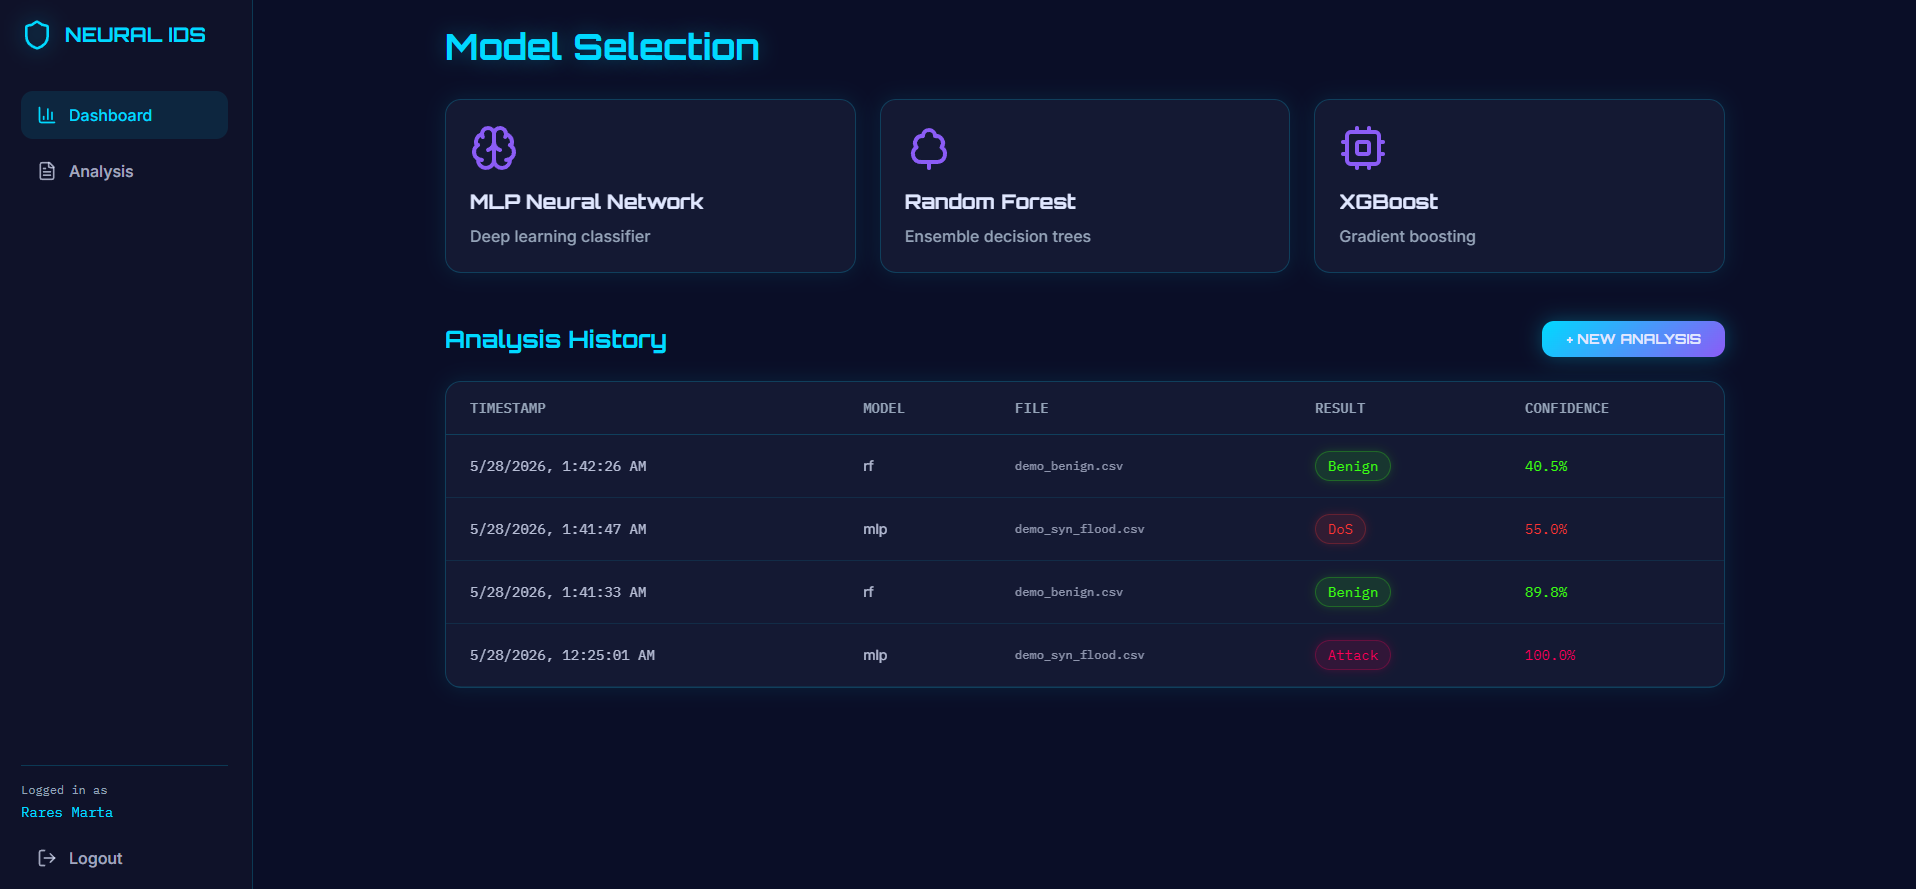
\includegraphics[width=0.78\textwidth]{figures/app_dashboard.png}
    \caption{NEURAL IDS dashboard after the acceptance runs. The analysis history table records four classification requests: the SYN-flood capture classified as Attack (near-certain binary confidence) and as DoS ($\approx$55\%) under different granularities, and the benign capture classified as Benign. The three model-selection cards at the top set the \texttt{model\_type} field of subsequent API calls. (Screenshot is illustrative; binary confidence is reported after temperature scaling in the text.)}
    \label{fig:app_dashboard}
\end{figure}

\par Figure~\ref{fig:app_attack} shows the detailed result screen for the SYN-flood capture classified under the temporal-split 8-class Random Forest variant. The top predicted class is \textbf{DoS} at 55\% mean confidence, with \textbf{DDoS} as the second-ranked class at 45\%. This is the expected result: a SYN flood is structurally a single-source volumetric attack, which the model correctly places in the DoS family (single-source high-rate flood) rather than DDoS (distributed multi-source flood). The processing time of 8~ms for 50 flows is well within the NFR-1 budget of 100~ms at p95.

\begin{figure}[htbp]
    \centering
    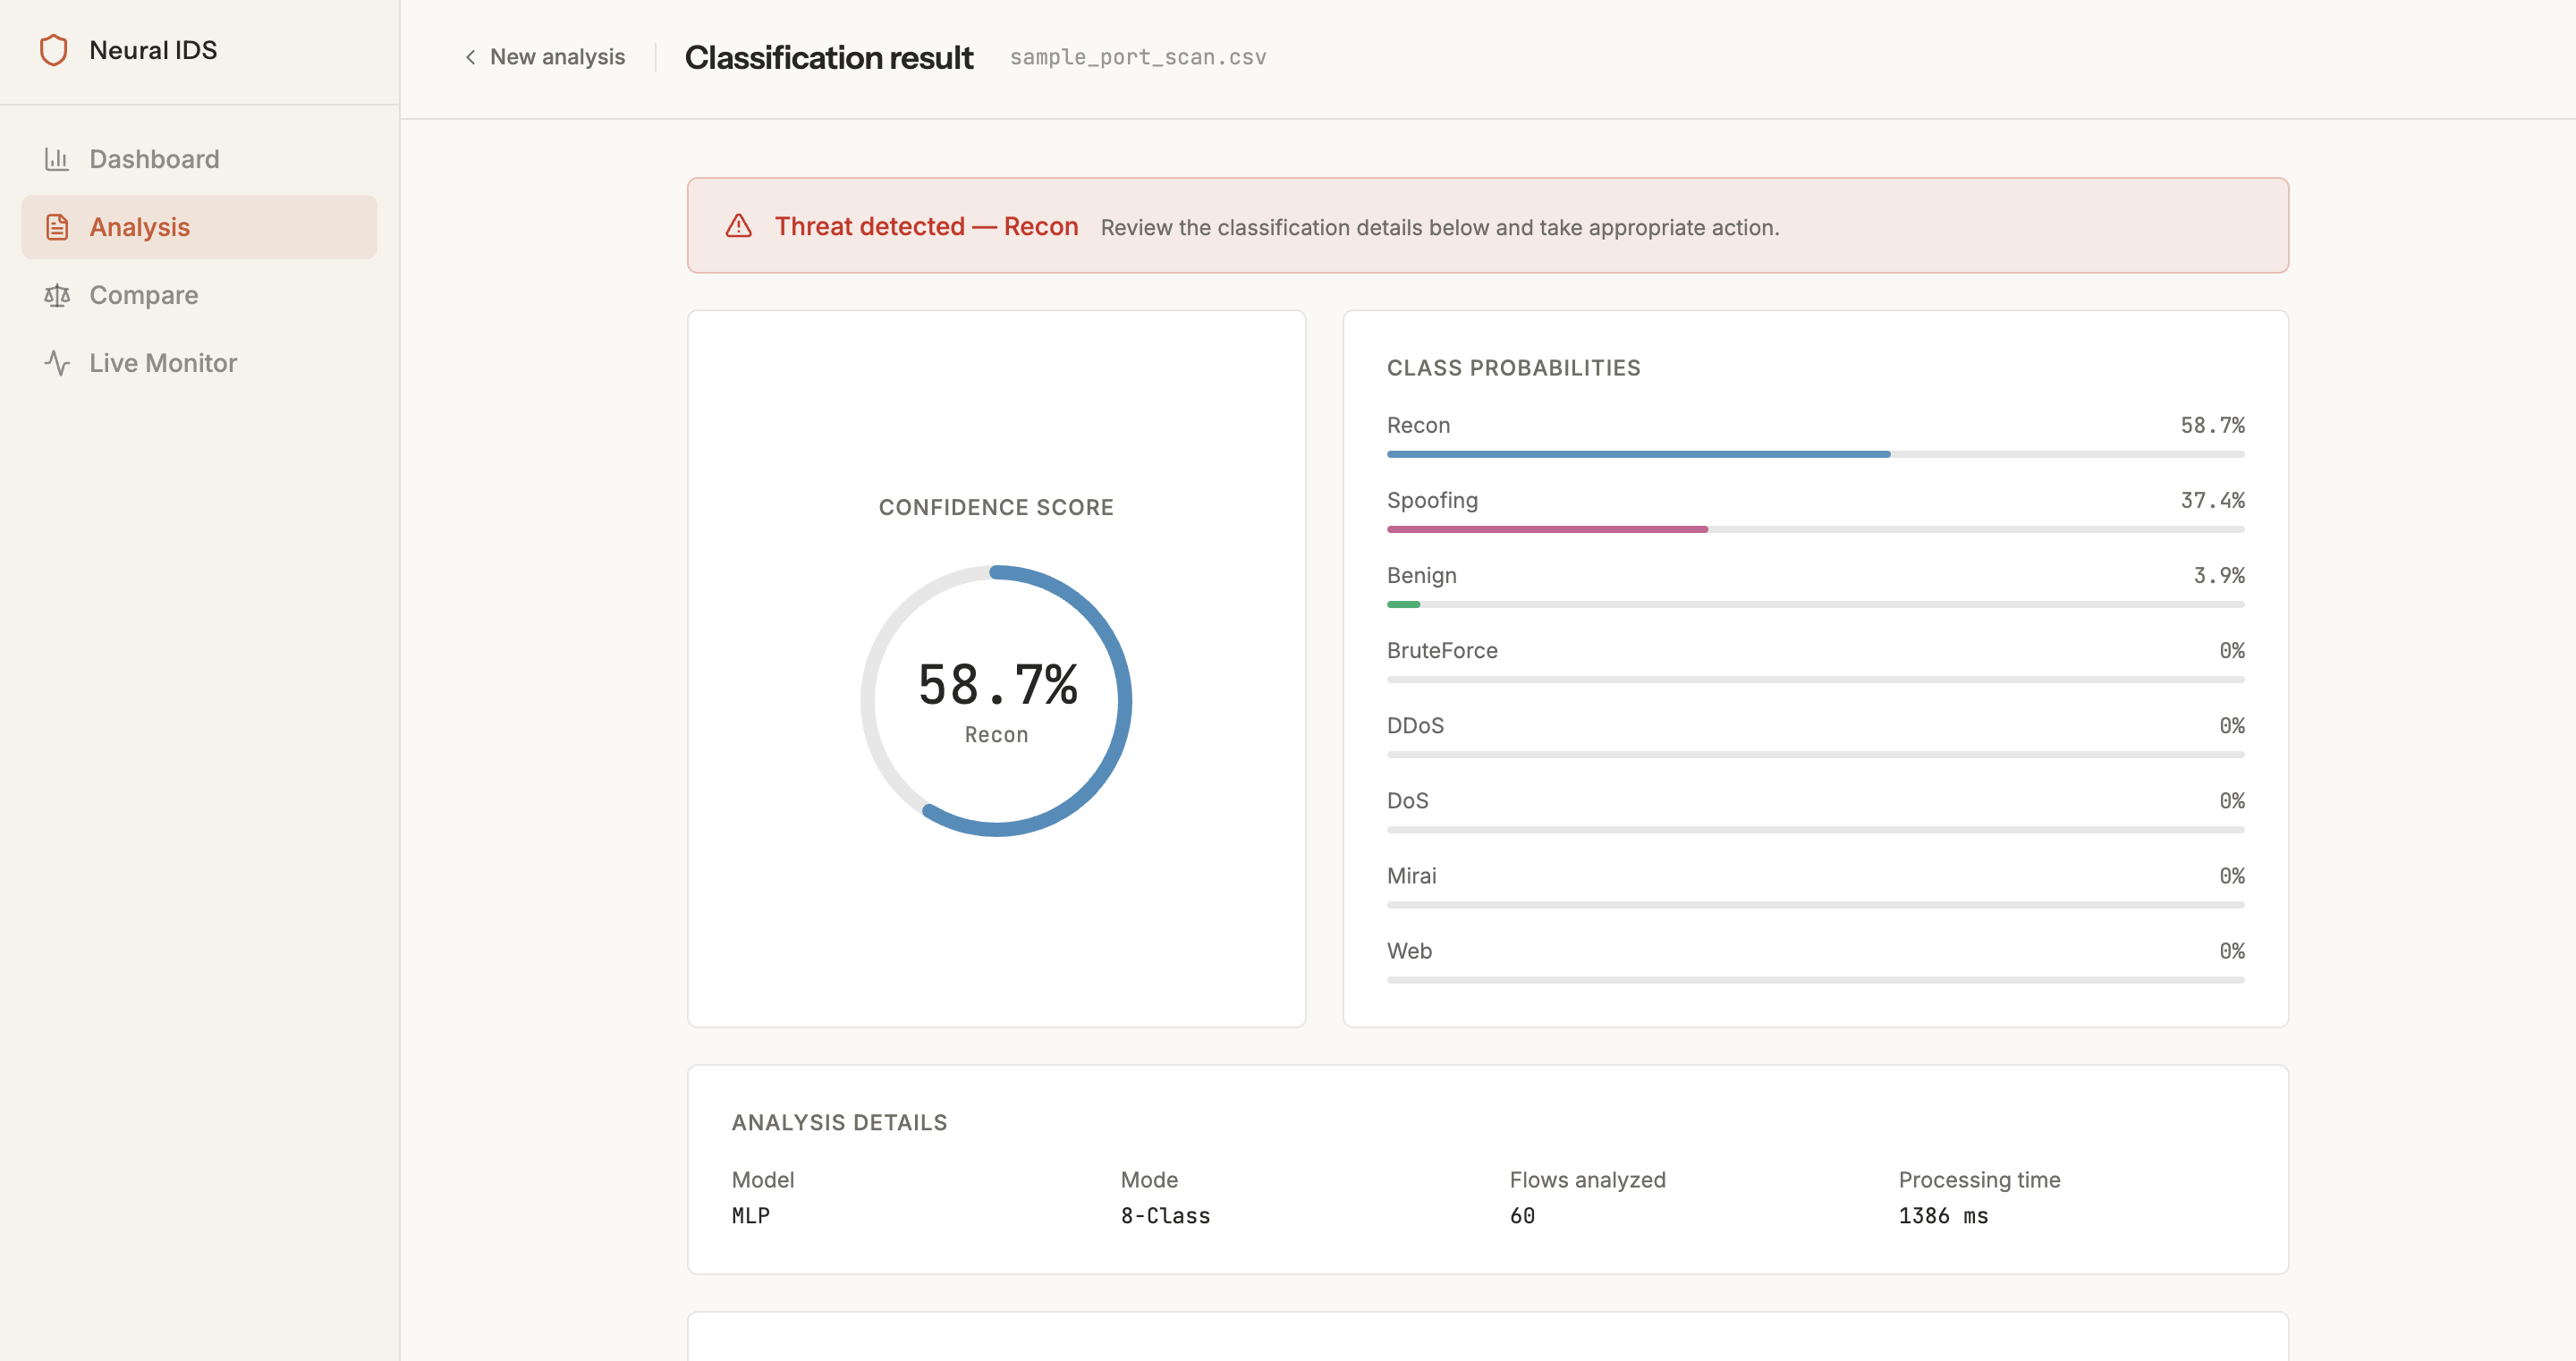
\includegraphics[width=0.50\textwidth]{figures/app_attack.png}
    \caption{Functional acceptance: SYN-flood capture classified under the temporal-split 8-class Random Forest variant. The alert banner confirms a threat detection; the class-probability panel ranks DoS (55\%) above DDoS (45\%), correctly identifying the single-source flood family. Analysis metadata (50 flows, 8~ms processing time) are shown in the lower panel.}
    \label{fig:app_attack}
\end{figure}
